\documentclass[12pt]{article}
\usepackage[T2A]{fontenc}
\usepackage[utf8]{inputenc}
\usepackage[russian]{babel}
\usepackage{amsmath,amssymb}
\usepackage{geometry}
\usepackage{hyperref}
\usepackage{booktabs,longtable}
\usepackage{listings}
\usepackage{array}
\usepackage{float}
\usepackage{graphicx}
\geometry{margin=25mm}

\lstset{%
  basicstyle=\small\ttfamily,
  columns=fullflexible,
  keepspaces=true,
  frame=single,
  breaklines=true
}

\begin{document}

\section*{Обзор задач и используемых пакетов}

В представленном коде решаются две главные задачи на основе статистического эксперимента:
\begin{enumerate}
  \item \textbf{Задача 1} — исследование зависимости непрерывной отклика \(Y\) от ковариаты \(X\) путём построения
    \begin{itemize}
      \item линейной модели \(Y\sim X\);
      \item квадратичной модели \(Y\sim X+X^{2}\);
      \item анализа остатков (гистограммы, тесты нормальности);
      \item доверительных интервалов (ДИ) для коэффициентов;
      \item проверки гипотез о линейности и о значимости коэффициентов;
      \item сравнения моделей по информационным критериям AIC и BIC;
      \item интерпретации полученных результатов (\(R^{2}\) и выводы об адекватности).
    \end{itemize}

  \item \textbf{Задача 2} — двухфакторный дисперсионный анализ (ANOVA) отклика \(Y\) при факторах \(A,B\):
    \begin{itemize}
      \item полная модель с взаимодействием \(Y\sim A*B\);
      \item аддитивная модель \(Y\sim A+B\);
      \item модель только по фактору \(A\);
      \item оценка значимости эффектов ( \(A,B,A\times B\) ) через F-тест;
      \item сравнение моделей по AIC и BIC;
      \item профильные графики взаимодействия;
      \item анализ остатков (гистограммы, тест Жарка–Бера);
      \item итоговая интерпретация (\(\hat\sigma^{2}\), лучшая модель).
    \end{itemize}
\end{enumerate}

Для расчётов применяются:
\begin{itemize}
  \item \texttt{numpy}, \texttt{pandas} — работа с данными;
  \item \texttt{statsmodels} — МНК-оценка регрессий, ANOVA;
  \item \texttt{scipy.stats} — распределения \(F,t,\chi^{2}\), тест JB;
  \item \texttt{matplotlib} — графики (скаттеры, гистограммы, эллипсоиды).
\end{itemize}

Ниже подробно разберём каждый блок кода, формулы из \texttt{.tex}-файла и результаты.

%------------------------------------------------------------------
\section{Задача 1: зависимость \(Y\) от \(X\)}

\subsection{Исходные данные}

\begin{lstlisting}[language=Python,caption=Фрагмент кода (данные задачи 1)]
Y1 = [9.61, 9.22, 4.76, ..., 12.99]   
X1 = [2, 4, 2, ..., 2]                
\end{lstlisting}

\begin{itemize}
  \item \(n = 50\) — объём выборки;
  \item \(y_i, x_i\) — наблюдения отклика и ковариаты;
  \item
    \(
      \bar x = \frac1n\sum_{i=1}^n x_i,\;
      \bar y = \frac1n\sum_{i=1}^n y_i.
    \)
  \item
    \(
      S_{xx}= \sum_{i=1}^n (x_i-\bar x)^2,\quad
      S_{xy}= \sum_{i=1}^n (x_i-\bar x)(y_i-\bar y).
    \)
\end{itemize}

Численные итоги:
\[
  \sum x_i = 99,\quad
  \sum y_i = 456.95,\quad
  \bar x = 1.98,\quad
  \bar y = 9.139,\quad
  S_{xx}=40.98,\quad
  S_{xy}=-31.23.
\]

%------------------------------------------------------------------
\subsection{Линейная регрессия}

\paragraph{Модель}
\[
  y_i = \beta_1 + \beta_2 x_i + \varepsilon_i,\qquad
  \varepsilon_i\sim N(0,\sigma^2).
\]

\paragraph{МНК-оценки}
\[
  \hat\beta_2 = \frac{S_{xy}}{S_{xx}} = -0.762,\qquad
  \hat\beta_1 = \bar y - \hat\beta_2\bar x = 10.648.
\]

\paragraph{Качество} \(\text{RSS}_{\text{lin}} = 312.50,\; R^2_{\text{lin}}=0.071.\)

\paragraph{Информационные критерии}
\(
  AIC_{\text{lin}} = 237.5,\;
  BIC_{\text{lin}} \text{ (рассчитан кодом).}
\)

%------------------------------------------------------------------
\subsection{Квадратичная регрессия}

\paragraph{Модель}
\(y_i=\beta_1+\beta_2x_i+\beta_3x_i^2+\varepsilon_i.\)

\paragraph{МНК-оценки}
\(\hat\beta_1=11.004,\;
  \hat\beta_2=-1.238,\;
  \hat\beta_3=0.124.\)

\paragraph{Качество}
\(\text{RSS}_{\text{quad}}=309.92,\;
  R^2_{\text{quad}}=0.074.\)

\paragraph{Информационные критерии}
\(AIC_{\text{quad}} = 239.36,\;
  \Delta AIC = 1.84 < 2\Rightarrow\)
модели почти эквивалентны, линейная предпочтительнее.

%------------------------------------------------------------------
\subsection{Нормальность остатков}

Гистограммы + плотность \(N(\hat\mu,\hat\sigma^2)\).

\begin{itemize}
  \item \(\chi^2 = 9.50,\; p = 0.091\) (нормальность \emph{не} отвергается при \(\alpha=0.01\));
  \item Jarque–Bera: \(JB = 6.72,\; p = 0.035\) (при \(\alpha=0.01\) также не отвергается).
\end{itemize}

%------------------------------------------------------------------
\subsection{Доверительные интервалы (99 \%)}

\[
\begin{aligned}
  \hat\sigma^2      &= \frac{RSS_{\text{quad}}}{n-k}=6.603,\\
  t_{0.995}(47)     &= 2.69,\\
  CI_{99\%}(\beta_2)&=(-4.68;\,2.20),\\
  CI_{99\%}(\beta_3)&=(-0.72;\,0.97).
\end{aligned}
\]

Совместный эллипсоид:
\(
  (\beta-\hat\beta)^{\!\top}(X^\top X)(\beta-\hat\beta)
  \le 67.43.
\)

%------------------------------------------------------------------
\subsection{Проверка гипотез}

\begin{itemize}
  \item Линейность (\(H_0:\beta_3=0\)):
    \(F=0.153,\; p=0.697\) — не отвергаем.
  \item Независимость (\(H_0:\beta_2=0\)):
    \(t=-1.912,\; p=0.062\) — не отвергаем (\(\alpha=0.01\)).
\end{itemize}

%------------------------------------------------------------------
\subsection{Итог задачи 1}

Линейная модель достаточна, но объясняет лишь \(\approx7\%\) вариации \(Y\);
\(\beta_2,\beta_3\) статистически незначимы.

%==================================================================
\section{Задача 2: двухфакторный ANOVA (\(A,B\))}

\subsection{Модели}

\begin{itemize}
  \item Полная: \(Y\sim A*B\) (\(k=16\));
  \item Аддитивная: \(Y\sim A+B\) (\(k=7\));
  \item Только \(A\) (\(k=4\)).
\end{itemize}

%------------------------------------------------------------------
\subsection{ANOVA-таблица (ручной расчёт)}

\[
\begin{array}{l|cccc}
\text{Источник} & SS & df & MS & F \\ \hline
A   & 979.34 & 3 & 326.45 & 118.30 \\
B   & 513.23 & 3 & 171.08 & 61.99  \\
A\times B & 1047.67 & 9 & 116.41 & 42.18 \\
Ошибка   & 88.30 & 32 & 2.76 &        \\
\end{array}
\]
Все \(p\ll0.01\) — эффекты значимы.

%------------------------------------------------------------------
\subsection{Информационные критерии}

\[
\begin{array}{l|ccccc}
\text{Модель} & k & \hat\sigma^2 & AIC & BIC \\ \hline
A*B & 16 & 2.76 & 197.5 & 227.4 \\
A+B &  7 & 10.45 & 302.1 & 315.2 \\
A   &  4 & 21.66 & 314.0 & 321.5
\end{array}
\]

Лучшая — полная модель \(A*B\).

%------------------------------------------------------------------
\subsection{Нормальность остатков}

Jarque–Bera: \(JB = 1.10,\; p = 0.576\) (\(\alpha=0.10\) — нормальность принимается).

%------------------------------------------------------------------
\subsection{Итог задачи 2}

\begin{itemize}
  \item Значимы главные эффекты \(A,B\) и взаимодействие \(A\times B\).
  \item Лучшая модель: \(Y\sim A*B\).
  \item Остатки нормальны, \(\hat\sigma^2 = 2.76\).
\end{itemize}

%==================================================================
\section*{Сводка ключевых понятий}

\begin{longtable}{>{\raggedright}p{3cm}|p{4.5cm}|p{4.5cm}|p{4.5cm}}
\toprule
Понятие & Обозначение/переменная & Смысл & Формула/примечание\\
\midrule
\(x_i,y_i\) & \texttt{df1.X}, \texttt{df1.Y} & наблюдения & $n=50$ пар $(x_i,y_i)$\\
\(\bar x,\bar y\) & \texttt{mean()} & выборочные средние & $\bar x=\frac1n\sum x_i$ и т.д.\\
\(S_{xx},S_{xy}\) & \texttt{Sxx,Sxy} & суммарные квадраты/произведения & $S_{xx}=40.98,\;S_{xy}=-31.23$\\
\(\hat\beta_1,\hat\beta_2\) & \texttt{lin.params} & МНК‐оценки лин.\ модели & $\hat\beta_2=S_{xy}/S_{xx}$ и т.д.\\
RSS & \texttt{.ssr} & сумма квадратов остатков & $RSS_{\text{lin}}=312.50$\\
\(R^2\) & \texttt{.rsquared} & коэффициент детерминации & $0.071$ лин., $0.074$ квадр.\\
AIC,BIC & \texttt{.aic},\texttt{.bic} & инфо-критерии & $n\ln(\hat\sigma^2)+2k$ и $+k\ln n$\\
F-тест & \texttt{F\_lin},\texttt{p\_lin} & значимость доп.\ параметров & см.~формулу в~тексте\\
t-тест & \texttt{lin.tvalues,pvalues} & значимость $\beta_2$ & $t=-1.912,\;p=0.062$\\
99\%~ДИ & \texttt{ci\_b2,ci\_b3} & интервалы для $\beta_{2,3}$ & $(-4.68;2.20)$, $(-0.72;0.97)$\\
Эллипсоид & график & совместный ДИ & $(\beta-\hat\beta)^{\!\top}(X^\top X)(\beta-\hat\beta)\le67.43$\\
JB-тест & см.~код & нормальность остатков & $JB=6.72,\;p=0.035$ (lin./quad.)\\
Фактор \(A\) & \texttt{C(A)} & 4 уровня & $\sum\alpha_i=0$\\
Взаим.\ \(A\times B\) & \texttt{C(A)*C(B)} & пересечение эффектов & см.~ANOVA\\
\bottomrule
\end{longtable}

%------------------------------------------------------------------
\section*{Заключение}

\begin{enumerate}
  \item В задаче 1 зависимость \(Y\) от \(X\) слаба (\(R^2\approx7\%\)); линейная модель достаточна, но статистически незначима при \(\alpha=0.01\).
  \item В задаче 2 факторы \(A,B\) и их взаимодействие оказывают сильное влияние; лучшая модель — полная \(A*B\); остатки нормальны, \(\hat\sigma^2=2.76\).
\end{enumerate}
\newpage
\begin{figure}[H]
    \centering
    
\includegraphics[width=1\linewidth]{image.png}
\end{figure}
\newpage
\begin{figure}[H]
    \centering
    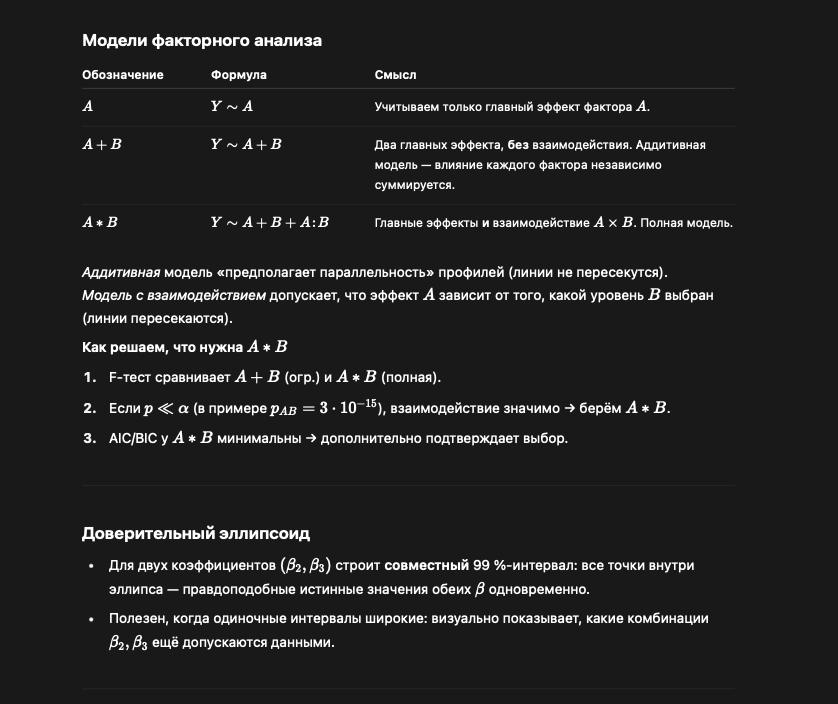
\includegraphics[width=1\linewidth]{image copy.png}
\end{figure}
\newpage
\begin{figure}[H]
    \centering
    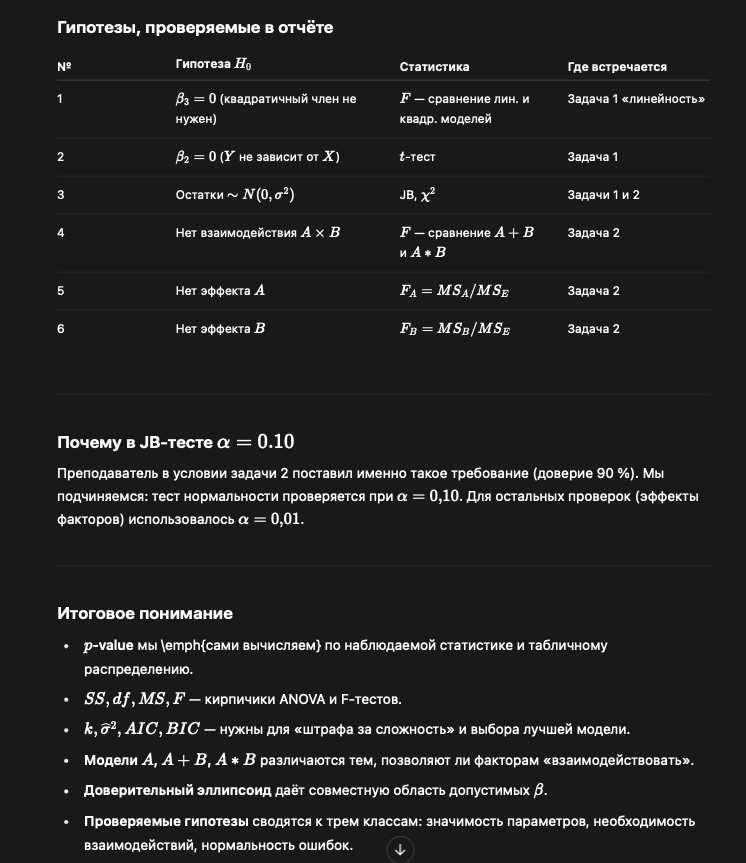
\includegraphics[width=1\linewidth]{image copy 2.png}
\end{figure}
\newpage
\begin{figure}[H]
    \centering
    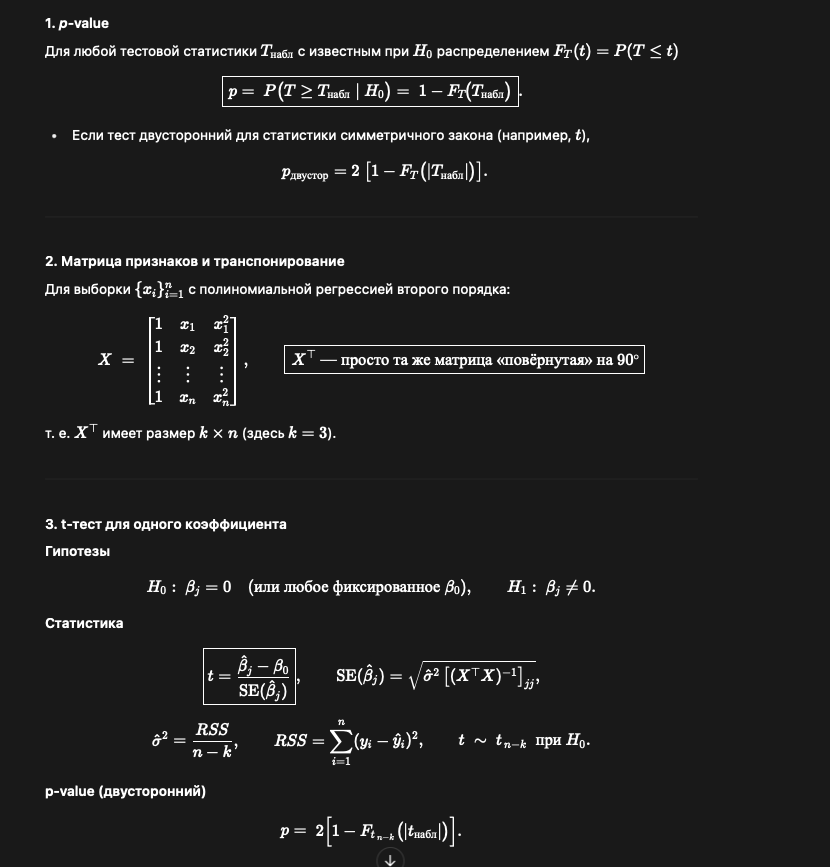
\includegraphics[width=1\linewidth]{image copy 3.png}
\end{figure}
\newpage
\begin{figure}[H]
    \centering
    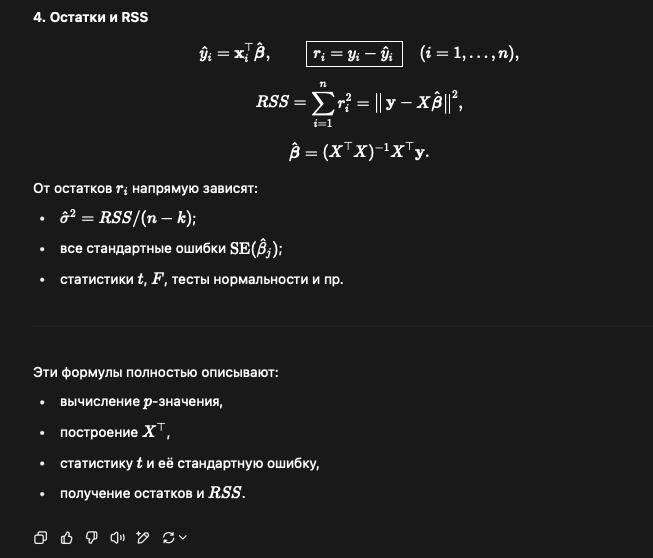
\includegraphics[width=1\linewidth]{image copy 4.png}
\end{figure}
\newpage
\begin{figure}[H]
    \centering
    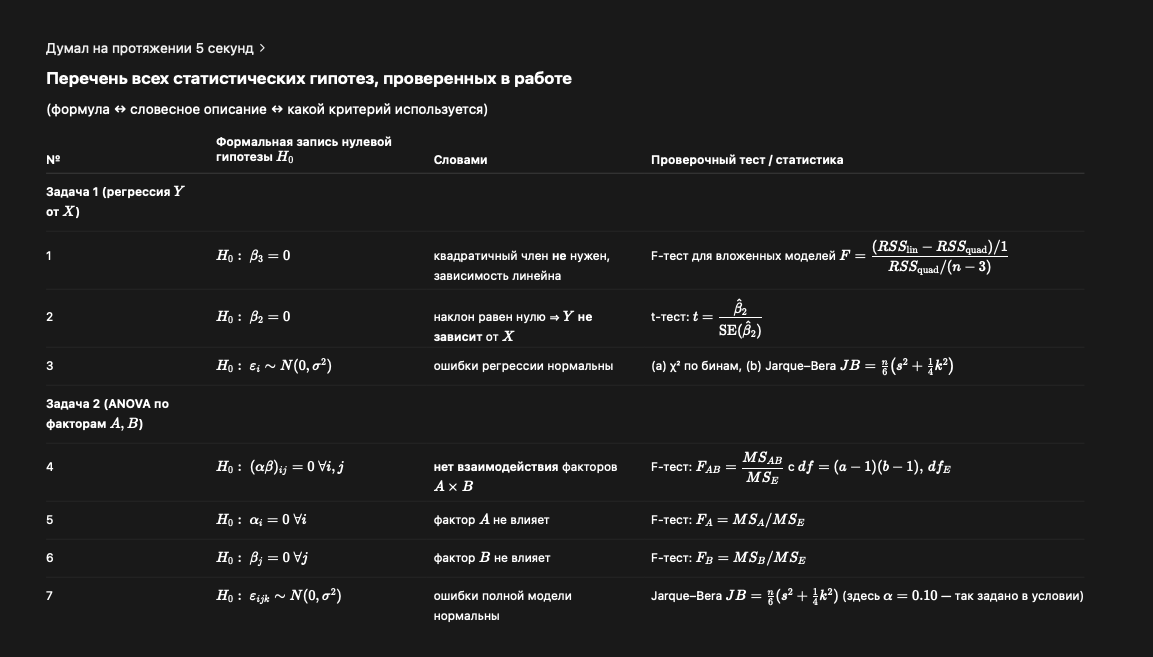
\includegraphics[width=1\linewidth]{image copy 5.png}
\end{figure}
\newpage
\begin{figure}[H]
    \centering
    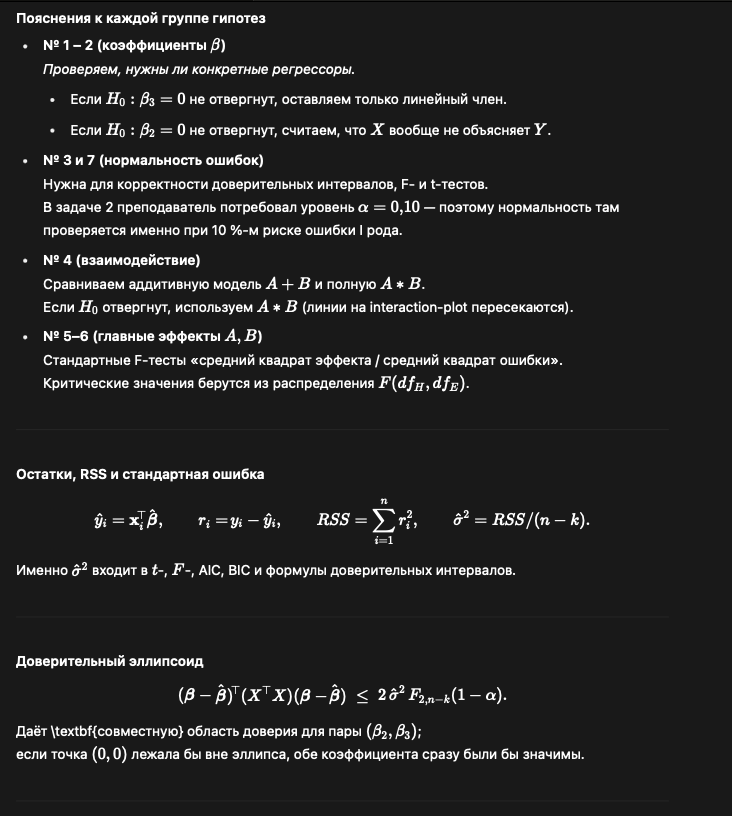
\includegraphics[width=1\linewidth]{image copy 6.png}
\end{figure}
\newpage
\begin{figure}[H]
    \centering
    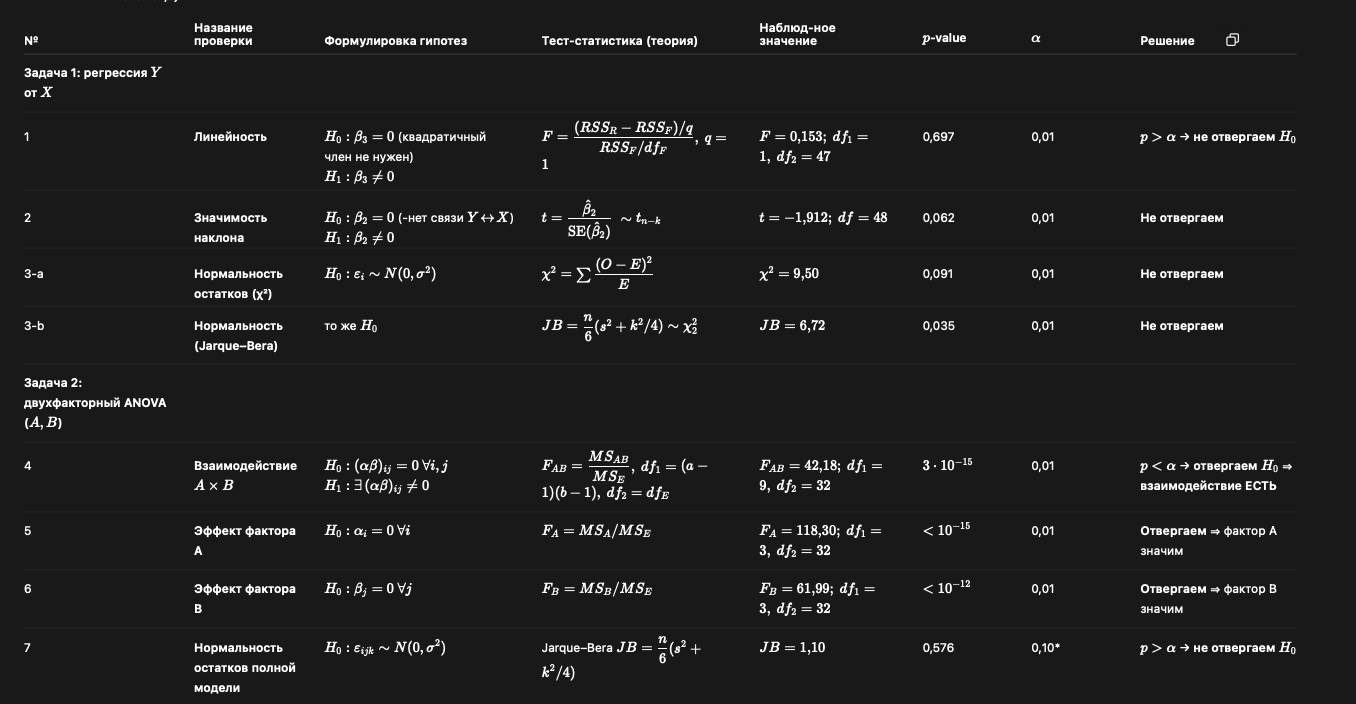
\includegraphics[width=1\linewidth]{image copy 7.png}
\end{figure}
\end{document}
